\documentclass[12pt]{beamer}

\definecolor{links}{HTML}{0D6957}
\hypersetup{colorlinks,linkcolor=,urlcolor=links}
\logo{
\includegraphics[width=1.5cm]{img/grt-t.png}}

\usepackage{amssymb,amsmath}
\usepackage[utf8x]{inputenc}
\usepackage{graphicx}
\usepackage{siunitx}
\usepackage{tikz}
\usepackage[normalem]{ulem}
\setcounter{secnumdepth}{0}
\usetheme{Berkeley}
\usecolortheme{seagull}
\usepackage{xcolor}

\def\myEmail{hxr@hx42.org}
\def\InternalGithub{erasche}

\def\myGithub{@\InternalGithub}
\def\myGithubUrl{https://github.com/\InternalGithub}
\def\myName{Helena Rasche}

\title[GRT]{
\includegraphics[width=4cm]{img/grt.png}}
\author[\myName\\ \color{gray} \myGpgFingerprint]{\myName}
\date[\today]{\today}

\begin{document}
\frame{\titlepage}

\section{Background}
\begin{frame}{The Need}
    \begin{itemize}
        \item Galaxies run on highly heterogeneous resources
        \item Jobs have highly heterogeneous resource requirements
        \item \ldots{}but we match them up manually or not at all.
    \end{itemize}
\end{frame}

\begin{frame}{The Solution}
    \begin{itemize}
        \item Just map them better! Obviously.
        \item Not trivial to do
        \item Local models may over-fit, or not fit at all. Who knows. We don't have data!
        \item So, time to collect it.
    \end{itemize}
\end{frame}

\section{GRT}
\begin{frame}{GRT}
    \begin{itemize}
        \item Galactic Radio Telescope, because it peers into Galaxies and extracts useful signals
        \item Collect job run metadata from individual Galaxies
        \begin{itemize}
            \item Strictly opt-in
            \item \# of cores during the run, dataset sizes, runtime, memory
            \item Other data points?
        \end{itemize}
    \end{itemize}
\end{frame}

\begin{frame}{Features}
    \begin{itemize}
        \item Collect Job Logs
        \begin{itemize}
            \item CPU Count
            \item Runtime
            \item Dataset Size
            \item Memory Usage
        \end{itemize}
        \item Analysis + Display Framework
        \item Side effect: Galactic Tool Registry
    \end{itemize}
\end{frame}

\begin{frame}{Roadmap}
    \begin{itemize}
        \item \sout{Collect Job Logs}
        \begin{itemize}
            \item CPU Count (1d, some small bug)
            \item \sout{Runtime}
            \item Dataset Size (1 month)
            \item Memory Usage (1d)
        \end{itemize}
        \item Analysis + Display Framework (post-gcc)
        \item \sout{Side effect: Galactic Tool Registry}
    \end{itemize}
\end{frame}

\section{Screenshots}
\begin{frame}{Galactic Directory}
    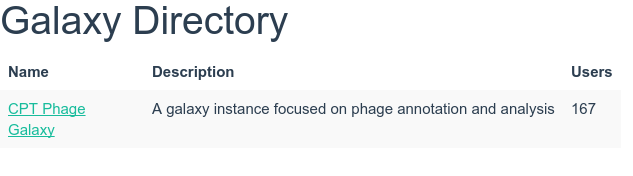
\includegraphics[width=\textwidth]{./img/directory.png}
\end{frame}

\begin{frame}{Administration}
    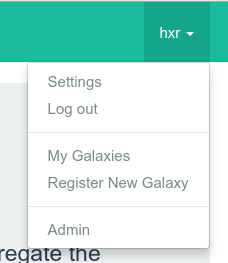
\includegraphics[height=.5\textheight]{./img/login-menu.png}
\end{frame}

\begin{frame}{Instance Metadata}
    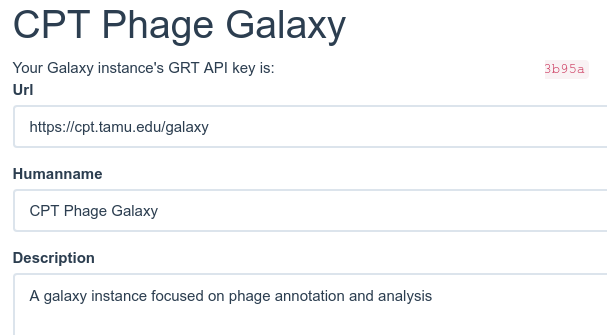
\includegraphics[width=\textwidth]{./img/instance-admin.png}
\end{frame}

\begin{frame}{Instance Info}
    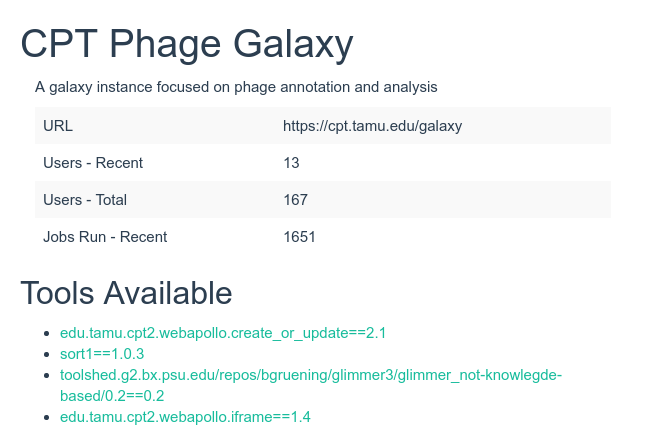
\includegraphics[width=\textwidth]{./img/instance-info.png}
\end{frame}

\begin{frame}{Tool Info}
    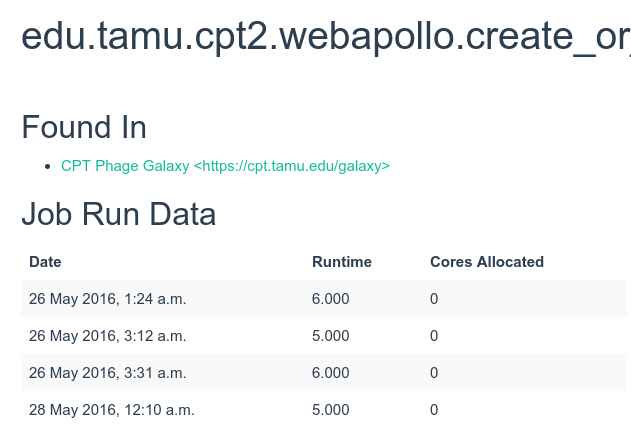
\includegraphics[width=\textwidth]{./img/tool-info.png}
\end{frame}

\section{Roadmap}
\begin{frame}{Going Forward}
    \begin{itemize}
        \item Fix CPU count issue (Hopefully by time of presentation)
        \item Integrate Jupyter server for crowd sourcing statistical analysis?
        \item If models can be built, then integrate \href{https://github.com/phac-nml/dynamic-tool-destination}{PHAC-NML's dynamic tool destinations}
        \item Galactic Tool / Analysis Directory (Where should I run my mapping job? Is there a public Galaxy for doing X?)
        \item Bragging? 
\includegraphics[width=5cm]{./img/badge.png}
    \end{itemize}
\end{frame}


\section{Q \& A}
\begin{frame}{Q \& A}

    \begin{center}
        Thank you! Questions? \\\ \\

        \begin{tabular}{rl}
            \color{gray} GPG Fingerprint  & \texttt{\myGpgA} \\
                                          & \texttt{\myGpgB} \\
            \color{gray} GitHub           & \href{\myGithubUrl}{\myGithub}\\
            \color{gray} Twitter          & \href{\myTwitterUrl}{\myTwitter}\\
            \color{gray} Work Email       & \href{mailto:\myEmail}{\myEmail}%
        \end{tabular}
    \end{center}
\end{frame}

\end{document}
